\documentclass[10pt,a4paper]{article}
\usepackage[T1]{fontenc}
\usepackage[scaled]{helvet}
\usepackage{cite}
\usepackage{url}
\usepackage{graphicx}
\usepackage{float}
\usepackage{amsmath}
\usepackage{amssymb}
\usepackage{fancyhdr}
\usepackage{lastpage}
\floatstyle{boxed} 
\restylefloat{figure}
\renewcommand*\familydefault{\sfdefault}
\title{Secondary Storage Systems and Parallel Architectures}
\author{David Lynch - david.lynch@raglansoftware.com }
\begin{document}
\maketitle
\begin{abstract}
This article focuses on secondary storage, which is not directly accessible by the CPU. Most common of these types is the hard disk drive. There is a special look at how hard disk drives can be arranged in different ways using the RAID standard. I also examine parallel architectures, introducing systems that contains multiple CPU's and different styles of CPU architecture. 
\end{abstract}
\section{Secondary Storage}
Secondary storage is deemed so because it is not directly accessible by the CPU. An intermediate area, such as a RAM buffer on a hard-disk controller, acts as a go-between. It is the responsibility of the {\bf disk controller} to facilitate interaction between the secondary disk, main memory and the CPU. A secondary storage is non-volatile memory that maintains it's state after power down. It is much less expensive relative to capacity than main memory, but the sacrifice made is in speed. Typical secondary storage devices operate with access times in the milliseconds. Common examples of secondary storage are magnetic disk as a floppy, or hard disk, DVD-ROM drives, Blu-Ray Drives and solid state USB drives.
\subsection{Hard Disk}
A hard drive is most informally a collection of high-capacity, circular magnetic disks that can store a large amount of information. The capacity of the hard drive is a function of the disk surface area and the density of bits on the surface area. A hard disk stores information serially on a non-removable disk with several {\bf platters}. Each platter is magnetizable on one or more surfaces. There are one or more {\bf read/write heads} per recording surface. Each of these platters is divided into concentric {\bf tracks}. The set of tracks equidistant from the centre is known as a {\bf cylinder}. Each track is divided into a sector of a fixed number of bytes, typically 256 to 4k in size. Like any magnetic media, some sectors of the hard disk become usable over time. In modern hard drives, sectors can be replaced by spare sectors that are included by not used until they are needed. The primary goal of the controller is to facilitate communication between the various sectors of the disk and the {\bf host controller} which in turn allows communication with the main system buses. A common form of hard disk controller and interface is Serial ATA. Other, older types, include SCSI and IDE. Typical server systems will also include a RAID controller, which we will discuss in detail later. This controller is responsible for the control of arrays that contain multiple disks in various configurations. 
\subsubsection{Performance Metrics}
Due to the number of mechanical movements, as well as the size of the disks themselves, and the logic that is required to manipulate them, hard drives are much slower than main memory in retrieving data. This is especially true from random access across the disk, where locality of reference principles often break down and caches on the disk controller become ineffective. \newline\newline The time required to move the heads from the current cylinder to the desired cylinder is the {\bf seek time}. The {\bf rotational delay} is the time required to find the desired sector once the correct cylinder is reached. The {\bf controller time} is the time required by the disk controller to perform address translation and other I/O operations. The {\bf disk transfer rate} is concerned with the quantity of data that can be transferred to and from the disk per second. These days this is measured in Megabytes or Gigabytes. Hard Drives exist today in the Gigabyte to Terabyte range, can spin at 10,000 rpm and can burst data up to 3GB per second. \newline\newline
From an application perspective, another important metric is {\bf Input-Output Operations Per Second} or IOPS. This measurement gives a fuller picture of the performance of a device under read and write than any of the metrics above in isolation. Random Read, Random Write, Sequential Read and Sequential Write IOPS can be further isolated to determine the performance characteristics of a particular disk. Hard disks with 100 total IOPS are common, and Solid State Disks with multiples of this are now becoming common. If I stream the contents of a video directly to the hard disk for saving, the sequential write IOPS are of interest. Conversely, if I'm running a database server that holds an encyclopaedia, the Random Read IOPS may be interesting, since as the number of requests for data increases, the speed of the response becomes important. 
\subsubsection{Other Characteristics}
Hard disk drives are mechanical in nature and therefore subject to failure over time. This can also mean hard disk drives are noisy. This may not be acceptable, for example, in a recording studio. They are also magnetic, which means they are prone to corruption. Some readers may be both old and young enough for a mobile phone to have caused havoc with an Iomega Zip cartridge, the same principle applies here. Further to this, due to the way the hard disk controller manages transfers between the disk and the computer, they are subject to fragmentation - lots more on this concept later on. In general, magnetic hard disk drives are really bad at doing anything that involves random access. 
\subsection{Solid State Disks}
These drives are becoming extremely popular for various reasons. The mechanics of a hard disk drive is replaced with the solid state nature of a NAND-type flash memory array. These drives operate in a way that is similar to main memory. They are advantageous over hard disk drives because they have negligible spin up times, low read latency times, have consistent performance characteristics across the disk and do not fragment. Further to this, they are not prone to physical shock or magnet corruption. However, they do have somewhat slower write cycles and a somewhat limited read-write life cycle meaning, they do not hold data consistently for as long as hard disk drives given comparable usage patterns. They are much more expensive than hard disk drive and therefore you will find them in smaller capacities. Lots of systems are now build whereby secondary storage is exclusively solid state, sometimes this is backed up by a traditional hard disk drive. In these configurations, the operating system often works off the solid state drive, improving system wide performance measurable. In the mixed case, the complimentary hard drive alleviates durability concerns. 
\subsection{RAID} 
RAID stands for Redundant Array of Independent Disks. RAID is used to mitigate the performance and reliability concerns of operating a single mechanical, magnetic disk in isolation. Multiple disks are configured in various ways, with the objective of increasing {\bf storage function}, {\bf performance} and {\bf redundancy}. RAID is very common in commercial servers, such as database servers, in particular in a cloud computing environment such as Amazon EC2, where inexpensive commodity hardware is used in bulk. There are three fundamental mechanisms that RAID uses to achieve it's goals. The following subsections outline these. 
\subsubsection{Data Striping}
Data striping is formally defined as segmentation of logically sequential data such that sequential accesses occur on different storage devices. If we configure two disks A and B to be stripped, sequential writes will be interleaved across both disks. If, for example, I need to write 10 bytes of data and an write operation consists of 1 byte, then the even bytes will appear on disk B and the odd ones on disk A, all in combined sequence. 
\subsubsection{Parity Bit}
A parity bit is a very simple form of error detection whereby the parity bit is set to 1 when the number of 1's in a given set of bits is odd. Party information for disk A may be stored on disk B and used to determine the whether the data in question is valid or not. A more advance form of parity checking is hamming code parity \ref{HAMMING-CODE}. This form adds error correction to the mix, allowing a full set of data to be reconstructed from a partial view of bits. 
\subsubsection{Mirroring}
Mirroring is the replication of logical disk volumes onto separate hard disk drives in real-time. If I have two disks A and B, then at any point in time after a complete write cycle, I have exactly the same data on disk A as I do on disk B. This is a form of redundancy, so if either disk fails, the data still endures. 
\subsubsection{RAID Level 0}
This level exhibits {\bf block level striping} with no parity and no mirroring. This improves performance, since we can concurrently be executing write cycles to two disks at a time. To a point of diminishing returns, the higher number of disks the greater the ability to write data concurrently and the the greater the overall bandwidth. However, as the number of disks increase, the chance of catastrophic failure increases also. 
\subsubsection{RAID Level 1}
This level is simply {\bf mirroring} without parity or striping. This decreases the chance of catastrophic failure and, again due potential concurrency, increases read access times. The sacrifice is, often marginal, decrease in write cycle time. 
\subsubsection{RAID Level 2}
Level one exhibits {\bf bit level striping} with \bf{hamming code parity}. Each sequential bit is on a different disk. To facilitate this, spindle rotation is synchronized. The parity data is stored on at least one of the disks and can be used to correct errors that are made on any disk over time. 
\subsubsection{RAID Level 3}
This level exhibits \{bf byte level striping} with {\bf dedicated parity}. A dedicated parity disk is required for this level. As with previous configurations, with dedicated parity any failure of the parity disk will leave the drive vulnerable and essential at RAID Level 0, except with byte level striping. 
\subsubsection{RAID Level 4}
Block level striping with dedicated parity.  
\subsubsection{RAID Level 5}
This level is one of the more popular due to the redundancy it provides. This resilience against failure is quite desirable, in particular in mission critical server systems. This level has block level striping with distributed parity. Since parity data is distributed across disks, it mitigates against failure of one or a number of the disks. When a disk fails, performance is merely degraded until it is repaired or replaced. 
\subsubsection{RAID Level 6}
To add another layer of redundancy, RAID level 6 has block level striping with double distributed parity. This gives full fault tolerance for two disk drive failures.
\subsection{Nested and Hybrid RAID}
In order to tune the level of reliability and performance, one can use multiple RAID configurations concurrently, either as a hybrid configuration or in a hierarchy. One of the most popular configurations for production data-base servers is RAID 1+0, commonly referred to as RAID 10. Specifically, RAID 10 is a set of mirrored disks in a striped set configuration. At least 4 disks are required for this configuration. The performance of Block level striping from RAID level 0 is complimented by the redundancy afforded by mirroring as is done in RAID level 1. Figure \ref{raid10} illustrates this configuration. Other hybrid configurations of RAID are also popular, for example, RAID 5+1, is a cost effective, performant system for read-oriented database systems. For further reading on RAID and the uses of RAID see. 
\begin{figure}
\caption{RAID 10 - A mirrored stripe configuration \cite{GEEKSRAID}}
\begin{center}
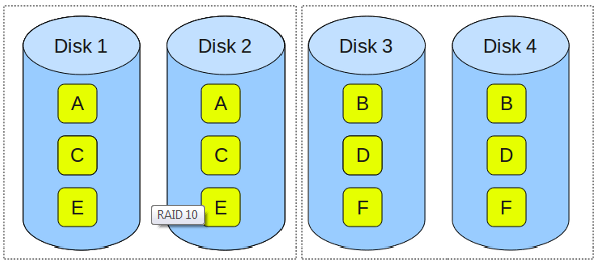
\includegraphics[scale=0.45]{../images/raid10.png}
\label{memory-h}
\end{center}
\end{figure}
\section{Parallel Architectures}
Thus far we have only discussed instructions executing serially. In all modern computer systems there is at least one form of parallelism acting at the core. Parallelism can simply be boiled down into executing multiple instructions, or parts of instructions at once. This can take the form of a single computer executing multiple programs in parallel, multiple cores (possibly distributed) executing multiple instructions in parallel, or single cores execution different stages of different instructions in parallel. In most modern computer systems aspects of all of the above feature. In short, parallelism can arise at the task level, the instruction level, or the machine level. 
\newline\newline
The Michael J. Flynn Taxonomy of Computer Architectures is still useful today for classifying differing types of architecture, particularly in the context of parallelism. He defined a parallel architecture as one that contains multiple interconnect \{bf processor elements}. The four classes of architecture discussed in the Taxonomy are as follows. 
\begin{itemize}
\item Single Instruction, Single Data (SISD)
\item Single Instruction, Multiple Data Stream (SIMD)
\item Multiple Instruction, Single Data (MISD)
\item Multiple Instruction, Multiple Data (Multi-Processors)
\end{itemize}


\bibliography{../biblio/techfundamentals.bib}{}
\bibliographystyle{plain}
\begin{center}
{\small \copyright  David Lynch 2012. Do not reproduce with written permission.}
\end{center}
\end{document}